\documentclass[a4paper,11pt]{jsarticle}


% 数式
\usepackage{amsmath,amsfonts}
\usepackage{bm}
% 画像
\usepackage[dvipdfmx]{graphicx}
\bibliographystyle{myjunsrt}
\renewcommand{\bibname}{References}


\begin{document}

\title{}
\author{}
\date{\today}
\maketitle

\section{tangent delta}

The basic equation for electromagnetic waves
when there is loss in the medium is as follows

\begin{equation}
  \mathrm{rot}(\frac{1}{\mu(\boldsymbol{r})}\mathrm{rot}\boldsymbol{E}) = -\mu_0 \mathrm{rot}(\frac{\partial H}{\partial t})
\end{equation}
\begin{equation}
  \mathrm{rot}(\frac{\partial H}{\partial t}) = \epsilon(\boldsymbol{r})\epsilon_0 \frac{\partial^2 E}{\partial t^2} + \frac{\partial J}{\partial t}
\end{equation}


We consider the characteristic value when there is loss in the medium.
When we consider the incidence of the time-varying factor $exp(j\omega t)$,
Maxwell's Equation can be written as follows.

\begin{equation} \label{eq:loss_electric_flux_density}
  \mathrm{rot} H = \epsilon \epsilon_0 \frac{\partial E}{\partial t} + \sigma \boldsymbol{E} = (j\omega\epsilon\epsilon_0 + \sigma)\boldsymbol{E}
\end{equation}

In this case, the right-hand side of Equation \ref{eq:loss_electric_flux_density}
is considered to arise from the flux density $\boldsymbol{D}$.

\begin{equation} \label{eq:electric_flux_density}
  \boldsymbol{D} = C\epsilon \epsilon_0 \boldsymbol{E}(\boldsymbol{r})exp(j\omega t)
\end{equation}

We derive $C=1 - j\sigma / \omega\epsilon\epsilon_0$ from the equation above.
Thus the electric flux density can be written as

\begin{equation} \label{eq:electric_flux_density_tangent_delta}
  \boldsymbol{D} = \dot{\epsilon} \epsilon_0 \boldsymbol{E} = \epsilon \epsilon_0 (1 - j\tan\delta)\boldsymbol{E}
\end{equation}

\begin{equation} \label{eq:epsilon_dot}
  \dot{\epsilon} = \epsilon (1 - j\tan\delta)
\end{equation}

\begin{equation} \label{eq:tangent_delta}
  \tan \delta = \frac{\sigma}{\omega\epsilon\epsilon_0}
\end{equation}

The parameter in Eq. \ref{eq:tangent_delta} is known as the loss tangent.
$\delta$を損失角という。高周波では、$\dot{\epsilon}$の実部の寄与が大きくなり、低周波では虚部の寄与が大きくなる。
言い換えると、誘電体に交流電場が加わったときにそのエネルギーの一部が熱となってしまう比率ともいえる。

\section{Skin effect}

In many of the experiments in this study, 
millimeter waves are blocked by copper plates.
The conductivity of the conductor $\sigma$ becomes very large,
and the amplitude damping constant $\alpha$ and the phase constant$\beta$
can be estimated as below.

\begin{equation}
  \alpha \approx \beta \approx \sqrt[]{\frac{\omega\mu\mu_0\sigma}{2}}
\end{equation}

This means that the attenuation of electromagnetic waves increases with increasing conductivity of $\sigma$
and the electromagnetic wave attenuates exponentially.
The depth δ at which the amplitude of the electromagnetic wave
at the surface is 1/e is called the skin depth, which can be expressed as below.

\begin{equation}
  \delta = \frac{1}{\alpha} = \sqrt[]{\frac{2}{\omega\mu\mu_0\sigma}}
\end{equation}

This indicates that the skin depth becomes shallower
as the frequency of the electromagnetic wave increases and the conductivity increases.
In this case, the current flows only near the surface of the copper plate,
which is called the skin effect.
The fact that current flows means that resistance exists,
and the skin resistance is written as follows.

\begin{equation}
  Re\{Z_W\} = \sqrt[]{\frac{\omega\mu\mu_0}{2}} = \frac{1}{\delta\sigma}
\end{equation}

Therefore copper plates can be used to effectively block millimeter waves.

\section{Snell's law}

At the boundary surfaces of different media, reflection and refraction of electromagnetic waves occur.
This is described by Snell's law.
This law can be derived using Maxwell's equations and boundary conditions.

媒質の境界面をx-y平面、各領域内で媒質がy方向に一様とする。
比誘電率と比透磁率を第一媒質に対して$\dot{\epsilon_1}$、$\mu_1$、
第二媒質に対して$\dot{\epsilon_2}$、$\mu_2$とする。
損失があるときの複素比誘電率を、次のようにおく。
$i$はそれぞれの媒質を表すので、1と2の値をとる。

\begin{equation}
  \dot{\epsilon_i} = \epsilon_i(1 - j\frac{\sigma_i}{\omega\epsilon_i\epsilon_0})
\end{equation}

ただし、$\sigma$は導電率、$\omega$は電磁波の角周波数、$\epsilon$は無損失時の比誘電率、
$\epsilon_0$は真空の誘電率を表す。
今回の比透磁率$\mu$は実数とする。
ここで各媒質の波数の大きさは$k$として以下のようになる。
$c$は真空中の光速である。

\begin{equation}
  k_i = \frac{\omega\sqrt[]{\dot{\epsilon_i}\mu_i}}{c}
\end{equation}

ここでTE波を例にSnellの法則を導き出す。
TE波は電界の振動方向が紙面に垂直であり、伝搬方向に電界成分を持たない。
紙面に垂直な方向は$y$軸なので、その電界を$E^i_y$として

\begin{equation}
  E^i_y = A_{iS}\exp[j(\omega t - \boldsymbol{k}_i\cdot\boldsymbol{r})]
\end{equation}

と書く。$A_{iS}$は電界振幅、$\boldsymbol{k}_i$は媒質中の波数ベクトル、
$\boldsymbol{r}$は波面の任意の点への位置ベクトルとなる。
添え字の$i$は3つの状態を持ち、入射・透過・反射をそれぞれ$i$、$t$、$r$で表す。

\section{全反射}

電磁波が密な媒質から疎な媒質に入射する場合、
入射角を徐々に大きくすると入射角より屈折角のほうが先に90度となる。
このとき、入射電磁波が透過することなく境界面で反射後に
すべて入射側に戻る現象を全反射という。

全反射時のTE波の透過電界成分は以下のように書ける。

\begin{equation}
  E^t_y = \exp[-j(\sqrt[]{\epsilon_1\mu_1}k_0\sin\theta_t)x]\exp\left(-\frac{z}{z_g}\right)
\end{equation}

\begin{equation}
  z_g = \frac{c}{\omega\sqrt[]{\epsilon_1\mu_1\sin^{2}\theta - \epsilon_2\mu_2}}
\end{equation}

$z_g$ は第二媒質への電界の侵入深さを表し、電磁波は境界面へわずかにしみでていることがわかる。
全反射時にも電磁波は境界面の反対側にもわずかに浸みだす。
この成分をevanescent波と呼ぶ。
電磁界の浸みこみと合わせて、反射点もずれる。
このずれのことをグースヘンヒェンシフトと呼ぶ。
誘電体導波路、光ファイバーを利用する際に重要となる。

電磁波は境界面の反対側にもわずかに浸みだすが、
注意しなければならないのはエネルギーは浸みださないことである。
振幅反射係数の和はすべて$1$となり、エネルギーもすべて反射する。

\begin{figure}
  \begin{center}
    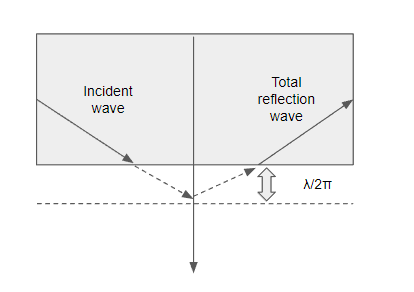
\includegraphics[clip, keepaspectratio, width=0.5\linewidth]{img/insertion_reflection_evanescence.png}
    \caption{evanescent成分の浸みだし}
    \label{fig:insertion_reflection_evanescent}
  \end{center}
\end{figure}


\section{電波の伝搬ロス}

自由空間を伝搬する電波の損失$L$は以下の式で表される。

\begin{equation}
  L = \left(\frac{4\pi d}{\lambda} \right)^2
\end{equation}

このとき$\lambda$は波長、$d$は距離となる。
例えば28GHzの電波を考えると波長は10mmなので、
0.25cm離れたところでは-49.3dBの減衰がみられる。
800MHz(波長375mm)の電波であれば、
同じ-49.3dBの減衰がみられるのは10m離れたところとなる。

TODO:画像追加

\section{リンクバジェット}

\section{曲がるアンテナ}

先行研究として株式会社NTTドコモが開発した曲がるアンテナが存在する
\cite{bending_antenna}。

\newpage
\addcontentsline{toc}{chapter}{\bibname}
\bibliography{common_bibliography}

\end{document}